\documentclass{beamer}

\usetheme{CambridgeUS}
\usecolortheme{orchid}

\usepackage{wrapfig}
\usepackage{siunitx}
\usepackage{inconsolata}
\usepackage{amsmath}
\usepackage{bm}
\usepackage{adjustbox}
\usepackage{nicefrac}

% Tikz
\usepackage{tikz}
\usetikzlibrary{positioning,shapes,arrows,calc,intersections}
\usepackage{pgfplots}
\usepgfplotslibrary{dateplot}
\pgfplotsset{compat=1.8}

\DeclareMathOperator{\spann}{span}

\begin{document}

\title[Div-conforming RBMs]{
  Fast Divergence-Conforming Reduced Basis Methods for Steady Navier-Stokes Flow
}
\author[E. Fonn]{
  E.~Fonn\inst{1,2} \and
  E.~H.~van Brummelen\inst{3} \and
  T.~Kvamsdal\inst{2,4} \and
  A.~Rasheed\inst{2} \and
  M.~S.~Siddiqui\inst{4}
}
\institute[SINTEF]{
  \inst{1}%
  \url{eivind.fonn@sintef.no}
  \and \inst{2}%
  Applied Mathematics, SINTEF ICT
  \and \inst{3}%
  Department of Mechanical Engineering, TU/e
  \and \inst{4}%
  Department of Mathematical Sciences, NTNU
}
\date[ECCM 2018]{}

\definecolor{darkblue}{HTML}{00688B}
\definecolor{darkgreen}{HTML}{6E8B3D}
\definecolor{cadet}{HTML}{DAE1FF}
\definecolor{salmon}{HTML}{FFB08A}

\titlegraphic{\includegraphics[width=0.3\textwidth]{common/sintef}}

\begin{frame}
  \titlepage
\end{frame}

\begin{frame}
  \frametitle{The stationary Navier-Stokes equations}

  \begin{alignat}{2}
    \label{eqn:ns-1}
    -\nu \Delta \bm u + (\bm u \cdot \nabla) \bm u + \nabla p &= \bm f && \qquad \text{in } \Omega, \\
    \label{eqn:ns-2}
    \nabla \cdot \bm u &= 0 && \qquad \text{in } \Omega, \\
    \label{eqn:ns-3}
    \bm u &= \bm g && \qquad \text{on } \Gamma_\text{D}, |\Gamma_D| > 0 \\
    \label{eqn:ns-4}
    -p \bm n + \nu (\nabla \bm u) \bm n &= \bm h && \qquad \text{on } \Gamma_\text{N}.
  \end{alignat}
\end{frame}

\begin{frame}
  \frametitle{Stationary NS: Weak formulation}

  Find $(\bm u, p)$ so that for all $(\bm w, q)$ it holds that
  \begin{align}
    a(\bm u, \bm w) + c(\bm u, \bm u, \bm w) + b(p, \bm w) &= d(\bm w), \label{eqn:var-1} \\
    b(q, \bm u) &= 0, \label{eqn:var-2}
  \end{align}
  Where
  \begin{align*}
    a(\bm u, \bm w) &= \nu \int_\Omega \nabla \bm u : \nabla \bm w,
    &b(p, \bm w) &= -\int_\Omega p \nabla \cdot \bm w, \\
    c(\bm u, \bm v, \bm w) &= \int_\Omega (\bm u \cdot \nabla) \bm v \cdot \bm w.
    &d(\bm w) &= \int_{\Gamma_\text{N}} \bm h \cdot \bm w + \int_{\Omega} \bm f \cdot \bm w,
  \end{align*}
\end{frame}

\begin{frame}
  \frametitle{Anatomy of a reduced system}

  Given reduced bases for velocity and pressure (V and P), the system matrix looks like this
  (at any point in the nonlinear solver stage).

  \begin{center}
    \begin{tikzpicture}[scale=1]
      \fill[cadet, draw=black, very thick, rounded corners=2mm] (0,-0.5) rectangle (0.95,-1.45);
      \fill[salmon, draw=black, densely dashed, rounded corners=2mm] (1,-0.5) rectangle (1.95,-1.45);
      \fill[salmon, draw=black, densely dashed, rounded corners=2mm] (0,-1.5) rectangle (0.95,-2.45);
      \node at (0.475,-0.975) {\large $VV$};
      \node at (1.475,-0.975) {\large $VP$};
      \node at (0.475,-1.975) {\large $PV$};
    \end{tikzpicture}
  \end{center}
\end{frame}

\begin{frame}
  \frametitle{An idea}

  \begin{itemize}
  \item In conventional solvers, pressure enters as a Lagrange multiplier to enforce the continuity
    equation.
  \item Incompatibilities between the velocity and pressure spaces are a frequent source of
    difficulties. (Also in reduced basis models; the VP matrix is often rank-deficient)
  \item If the velocity space were \emph{a priori} divergence free, you wouldn't need a pressure
    field at all. You could solve directly for velocity and, if necessary, reconstruct the pressure
    in post.
  \end{itemize}

  Enter: Isogeometric Analysis (IGA).
\end{frame}

\begin{frame}
  \frametitle{IGA}

  B-Spline basis functions.

  \begin{center}
    \begin{tikzpicture}
      \begin{axis}[
        xlabel={$x$},
        ylabel={$b(x)$},
        xmin=0, xmax=10,
        ymin=0.001,
        width=0.9\textwidth,
        height=0.5\textwidth,
        axis lines=left,
        ticks=none,
        ]
        \only<1>{
        \addplot[blue, thick] table[x index={0}, y index={1}]{data/linbasis.csv};
        \addplot[red, thick] table[x index={0}, y index={2}]{data/linbasis.csv};
        \addplot[teal, thick] table[x index={0}, y index={3}]{data/linbasis.csv};
        \addplot[magenta, thick] table[x index={0}, y index={4}]{data/linbasis.csv};
        \addplot[black, thick] table[x index={0}, y index={5}]{data/linbasis.csv};
        \addplot[cyan, thick] table[x index={0}, y index={6}]{data/linbasis.csv};
        \addplot[lime, thick] table[x index={0}, y index={7}]{data/linbasis.csv};
        \addplot[violet, thick] table[x index={0}, y index={8}]{data/linbasis.csv};
        \addplot[orange, thick] table[x index={0}, y index={9}]{data/linbasis.csv};
        \addplot[pink, thick] table[x index={0}, y index={10}]{data/linbasis.csv};
        \addplot[darkgray, thick] table[x index={0}, y index={11}]{data/linbasis.csv};
        }
        \only<2>{
        \addplot[blue, thick] table[x index={0}, y index={1}]{data/quadbasis.csv};
        \addplot[red, thick] table[x index={0}, y index={2}]{data/quadbasis.csv};
        \addplot[teal, thick] table[x index={0}, y index={3}]{data/quadbasis.csv};
        \addplot[magenta, thick] table[x index={0}, y index={4}]{data/quadbasis.csv};
        \addplot[black, thick] table[x index={0}, y index={5}]{data/quadbasis.csv};
        \addplot[cyan, thick] table[x index={0}, y index={6}]{data/quadbasis.csv};
        \addplot[lime, thick] table[x index={0}, y index={7}]{data/quadbasis.csv};
        \addplot[violet, thick] table[x index={0}, y index={8}]{data/quadbasis.csv};
        \addplot[orange, thick] table[x index={0}, y index={9}]{data/quadbasis.csv};
        \addplot[pink, thick] table[x index={0}, y index={10}]{data/quadbasis.csv};
        \addplot[darkgray, thick] table[x index={0}, y index={11}]{data/quadbasis.csv};
        \addplot[blue, thick] table[x index={0}, y index={12}]{data/quadbasis.csv};
        }
        \only<3>{
        \addplot[blue, thick] table[x index={0}, y index={1}]{data/cubasis.csv};
        \addplot[red, thick] table[x index={0}, y index={2}]{data/cubasis.csv};
        \addplot[teal, thick] table[x index={0}, y index={3}]{data/cubasis.csv};
        \addplot[magenta, thick] table[x index={0}, y index={4}]{data/cubasis.csv};
        \addplot[black, thick] table[x index={0}, y index={5}]{data/cubasis.csv};
        \addplot[cyan, thick] table[x index={0}, y index={6}]{data/cubasis.csv};
        \addplot[lime, thick] table[x index={0}, y index={7}]{data/cubasis.csv};
        \addplot[violet, thick] table[x index={0}, y index={8}]{data/cubasis.csv};
        \addplot[orange, thick] table[x index={0}, y index={9}]{data/cubasis.csv};
        \addplot[pink, thick] table[x index={0}, y index={10}]{data/cubasis.csv};
        \addplot[darkgray, thick] table[x index={0}, y index={11}]{data/cubasis.csv};
        \addplot[blue, thick] table[x index={0}, y index={12}]{data/cubasis.csv};
        \addplot[red, thick] table[x index={0}, y index={13}]{data/cubasis.csv};
        }
        \only<4>{
        \addplot[blue, thick] table[x index={0}, y index={1}]{data/quartbasis.csv};
        \addplot[red, thick] table[x index={0}, y index={2}]{data/quartbasis.csv};
        \addplot[teal, thick] table[x index={0}, y index={3}]{data/quartbasis.csv};
        \addplot[magenta, thick] table[x index={0}, y index={4}]{data/quartbasis.csv};
        \addplot[black, thick] table[x index={0}, y index={5}]{data/quartbasis.csv};
        \addplot[cyan, thick] table[x index={0}, y index={6}]{data/quartbasis.csv};
        \addplot[lime, thick] table[x index={0}, y index={7}]{data/quartbasis.csv};
        \addplot[violet, thick] table[x index={0}, y index={8}]{data/quartbasis.csv};
        \addplot[orange, thick] table[x index={0}, y index={9}]{data/quartbasis.csv};
        \addplot[pink, thick] table[x index={0}, y index={10}]{data/quartbasis.csv};
        \addplot[darkgray, thick] table[x index={0}, y index={11}]{data/quartbasis.csv};
        \addplot[blue, thick] table[x index={0}, y index={12}]{data/quartbasis.csv};
        \addplot[red, thick] table[x index={0}, y index={13}]{data/quartbasis.csv};
        \addplot[teal, thick] table[x index={0}, y index={14}]{data/quartbasis.csv};
        }
      \end{axis}
    \end{tikzpicture}
  \end{center}
\end{frame}

\begin{frame}
  \frametitle{Divergence-conforming methods}

  This way it's easy to create a divergence-conforming method on a
  rectilinear grid:

  \begin{itemize}
  \item $v_1$: degree $(r+1,r)$ and continuity $(C^r, C^{r-1})$
  \item $v_2$: degree $(r,r+1)$ and continuity $(C^{r-1}, C^r)$
  \item $p$: degree $(r,r)$ and continuity $(C^{r-1}, C^{r-1})$
  \end{itemize}

  Then, $\nabla \cdot V = P$, and the inf-sup conditions are trivially satisfied.
\end{frame}

\begin{frame}
  \frametitle{Geometry mapping}

  We are usually not interested in rectangular domains, and the divergence-conforming property is
  not generally preserved using a pointwise velocity mapping:
  \[
    \bm v = \hat{\bm v} \circ \pi^{-1}
  \]
  where $\pi : \hat{\Omega}_{\text{param}} \to \hat{\Omega}$. Instead, the Piola mapping does the trick:
  \[
    \bm v = \frac{\bm J}{|\bm J|} (\hat{\bm v} \circ \pi^{-1})
  \]
  where $\bm J$ is the Jacobian of $\pi$.
\end{frame}

\begin{frame}
  \frametitle{Geometry mapping (cont.)}

  We use the same idea to map velocity fields from the reference domain $\hat{\Omega}$ to
  parametrized geometries $\Omega(\bm \mu)$.
  \\~\\
  This generally has the effect of massively complicating affine representations,
  \[
    \bm A_h(\bm \mu) = \textstyle \sum_i \xi_i(\bm \mu) \bm A_i, \qquad
    \bm f_h(\bm \mu) = \textstyle \sum_i \chi_i(\bm \mu) \bm f_i
  \]
  however we intend to justify the \emph{means} by the \emph{end}.
\end{frame}

\begin{frame}
  \frametitle{Divergence-free basis}

  \begin{center}
    \begin{tikzpicture}[
      block/.style={
        minimum width=40mm,
        minimum height=8mm,
        align=center,
        rounded corners,
        fill=cadet,
        draw=darkblue,
      }
      ]
      \node[block] (HIFI) at (0,6.4) {Hi-Fi solutions};
      \node[block] (RGEOM) at (0,5.2) {Reference geometry};
      \node[block] (UNLIF) at (0,4) {Unlifted solutions};
      \node[block,fill=salmon] (POD) at (0,2.8) {POD};
      \node[block] (RB) at (0,1.6) {Reduced basis};

      \draw[->] (HIFI.south) -- (RGEOM.north);
      \draw[->] (RGEOM.south) -- (UNLIF.north);
      \draw[->] (UNLIF.south) -- (POD.north);
      \draw[->] (POD.south) -- (RB.north);

      \only<2-6>{\draw[->, very thick, white] (-3.5,5.2) -- (HIFI.west);}
      \only<2>{\draw[->, very thick, darkblue] (3.5,6.4) -- (HIFI.east);}
      \only<3>{\draw[->, very thick, darkblue] (3.5,5.2) -- (RGEOM.east);}
      \only<4>{\draw[->, very thick, darkblue] (3.5,4) -- (UNLIF.east);}
      \only<5>{\draw[->, very thick, darkblue] (3.5,2.8) -- (POD.east);}
      \only<6>{\draw[->, very thick, darkblue] (3.5,1.6) -- (RB.east);}
    \end{tikzpicture}
  \end{center}
\end{frame}

\begin{frame}
  \frametitle{Divergence-free basis}

  \begin{itemize}
  \item The mapping from reference to physical geometry needs to preserve divergence-free functions
    (the Piola mapping).
  \item Lifting functions must also be divergence-free.
  \item That's it!
  \end{itemize}
\end{frame}

\begin{frame}
  \frametitle{Anatomy of a divergence-free reduced system}

  \begin{center}
    \begin{tikzpicture}[scale=1]
      \fill[cadet, draw=black, very thick, rounded corners=2mm] (0,-0.5) rectangle (0.95,-1.45);
      \fill[salmon, draw=black, densely dashed, rounded corners=2mm] (1,-0.5) rectangle (1.95,-1.45);
      \fill[salmon, draw=black, densely dashed, rounded corners=2mm] (0,-1.5) rectangle (0.95,-2.45);
      \node at (0.475,-0.975) {\large $VV$};
      \node at (1.475,-0.975) {\large $VP$};
      \node at (0.475,-1.975) {\large $PV$};

      \node at (2.4,-1.5) {$\Rightarrow$};

      \fill[cadet, draw=black, very thick, rounded corners=2mm] (3,-0.5) rectangle (3.95,-1.45);
      \draw[black, densely dashed, rounded corners=2mm] (4,-0.5) rectangle (4.95,-1.45);
      \draw[black, densely dashed, rounded corners=2mm] (3,-1.5) rectangle (3.95,-2.45);
      \node at (3.475,-0.975) {\large $VV$};
    \end{tikzpicture}
  \end{center}

  A true velocity-only formulation is achieved.
\end{frame}

\begin{frame}
  \frametitle{Supremizers}

  To solve for pressure, we leverage a technique from Ballarin et.~al.~(2015). There, the velocity
  space is enriched with \emph{supremizers} to stabilize and control the LBB condition.

  \begin{center}
    \begin{tikzpicture}[scale=1]
      \fill[cadet, draw=black, very thick, rounded corners=2mm] (0,-0.5) rectangle (0.95,-1.45);
      \fill[salmon, draw=black, densely dashed, rounded corners=2mm] (1,-0.5) rectangle (1.95,-1.45);
      \fill[salmon, draw=black, densely dashed, rounded corners=2mm] (0,-1.5) rectangle (0.95,-2.45);
      \node at (0.475,-0.975) {\large $VV$};
      \node at (1.475,-0.975) {\large $VP$};
      \node at (0.475,-1.975) {\large $PV$};

      \node at (2.4,-1.5) {$\Rightarrow$};

      \fill[cadet, draw=black, very thick, rounded corners=2mm] (3,0) rectangle (3.95,-0.95);
      \fill[cadet, draw=black, very thick, rounded corners=2mm] (4,0) rectangle (4.95,-0.95);
      \fill[cadet, draw=black, very thick, rounded corners=2mm] (3,-1) rectangle (3.95,-1.95);
      \fill[cadet, draw=black, very thick, rounded corners=2mm] (4,-1) rectangle (4.95,-1.95);
      \fill[salmon, draw=black, densely dashed, rounded corners=2mm] (5,0) rectangle (5.95,-0.95);
      \fill[salmon, draw=black, densely dashed, rounded corners=2mm] (3,-2) rectangle (3.95,-2.95);
      \fill[salmon, draw=black, very thick, rounded corners=2mm] (5,-1) rectangle (5.95,-1.95);
      \fill[salmon, draw=black, very thick, rounded corners=2mm] (4,-2) rectangle (4.95,-2.95);
      \node at (3.475,-0.475) {\large $VV$};
      \node at (4.475,-0.475) {\large $VS$};
      \node at (5.475,-0.475) {\large $VP$};
      \node at (3.475,-1.475) {\large $SV$};
      \node at (4.475,-1.475) {\large $SS$};
      \node at (5.475,-1.475) {\large $SP$};
      \node at (3.475,-2.475) {\large $PV$};
      \node at (4.475,-2.475) {\large $PS$};
    \end{tikzpicture}
  \end{center}
  Supremizers are maximizers of the ``sup'' part of the inf-sup expression.
\end{frame}

\begin{frame}
  \frametitle{Supremizers (cont.)}

  For the same reason, supremizers are natural test functions when solving the momentum equation
  for pressure.

  \begin{center}
    \begin{tikzpicture}[scale=1]
      \fill[cadet, draw=black, very thick, rounded corners=2mm] (7,-0.5) rectangle (7.95,-1.45);
      \draw[black, densely dashed, rounded corners=2mm] (8,-0.5) rectangle (8.95,-1.45);
      \draw[black, densely dashed, rounded corners=2mm] (7,-1.5) rectangle (7.95,-2.45);
      \node at (7.475,-0.975) {\large $VV$};

      \node at (9.4,-1.5) {$\Rightarrow$};

      \fill[cadet, draw=black, very thick, rounded corners=2mm] (10,0) rectangle (10.95,-0.95);
      \fill[cadet, draw=black, very thick, rounded corners=2mm] (11,0) rectangle (11.95,-0.95);
      \fill[cadet, draw=black, very thick, rounded corners=2mm] (10,-1) rectangle (10.95,-1.95);
      \fill[cadet, draw=black, very thick, rounded corners=2mm] (11,-1) rectangle (11.95,-1.95);
      \draw[black, densely dashed, rounded corners=2mm] (12,0) rectangle (12.95,-0.95);
      \draw[black, densely dashed, rounded corners=2mm] (10,-2) rectangle (10.95,-2.95);
      \fill[salmon, draw=black, very thick, rounded corners=2mm] (12,-1) rectangle (12.95,-1.95);
      \fill[salmon, draw=black, very thick, rounded corners=2mm] (11,-2) rectangle (11.95,-2.95);
      \node at (10.475,-0.475) {\large $VV$};
      \node at (11.475,-0.475) {\large $VS$};
      \node at (10.475,-1.475) {\large $SV$};
      \node at (11.475,-1.475) {\large $SS$};
      \node at (12.475,-1.475) {\large $SP$};
      \node at (11.475,-2.475) {\large $PS$};
    \end{tikzpicture}
  \end{center}

  Note the block-triangular structure. (Also, the last equation is trivial.)
\end{frame}

\begin{frame}
  \frametitle{Block solver structure}

  \[
    B_{ps} \bm s = \bm 0 \quad \Rightarrow \quad \bm s = \bm 0
  \]

  So supremizers are truly test functions, have no influence on the solution.

  \begin{align*}
    \bm s &= \bm 0 \\
    \bm A_{vv} \bm v &= \bm f_{v} \\
    \bm B_{sp} \bm p &= \bm f_{p} - A_{sv} \bm v
  \end{align*}

  Solve two systems of size $M$ instead of one system of size $3M$.
\end{frame}

\begin{frame}
  \frametitle{Flow around airfoil}

  \begin{center}
    \begin{tikzpicture}
      \draw[densely dotted, thick] (0,-3) arc (-90:90:3);
      \draw[thick] (0,3) arc (90:270:3);
      \draw[->] (-3,0) -- (-2.2,0);
      \draw[->] (-2.93,0.6) -- (-2.13,0.6);
      \draw[->] (-2.75,1.2) -- (-1.95,1.2);
      \draw[->] (-2.40,1.8) -- (-1.60,1.8);
      \draw[->] (-1.80,2.4) -- (-1.00,2.4);
      \draw[->] (-2.93,-0.6) -- (-2.13,-0.6);
      \draw[->] (-2.75,-1.2) -- (-1.95,-1.2);
      \draw[->] (-2.40,-1.8) -- (-1.60,-1.8);
      \draw[->] (-1.80,-2.4) -- (-1.00,-2.4);
      \node[anchor=east] at (-3,0) {$\bm u_\infty$};
      \draw[->] (1.6,0) arc (0:30:1.6);
      \draw[->] (1.6,0) arc (0:-30:1.6);
      \node[anchor=west] at (1.6,0) {$\varphi$};
      \begin{scope}[scale=0.3, shift={(-3,-1.4)}]
        \begin{axis}[xmin=-0.01, xmax=1.01, ymin=-0.2, ymax=0.2, unit vector ratio*=1 1, axis lines=none]
          \addplot[black, line width=2.5]
          table[x index={0}, y index={1}]{data/NACApts.dat};
        \end{axis}
      \end{scope}
      \begin{scope}[scale=0.3, rotate=30, shift={(-3,-1.5)}]
        \begin{axis}[xmin=-0.01, xmax=1.01, ymin=-0.2, ymax=0.2, unit vector ratio*=1 1, axis lines=none]
          \addplot[black, line width=1.5, dotted]
          table[x index={0}, y index={1}]{data/NACApts.dat};
        \end{axis}
      \end{scope}
      \begin{scope}[scale=0.3, rotate=-30, shift={(-3,-1.3)}]
        \begin{axis}[xmin=-0.01, xmax=1.01, ymin=-0.2, ymax=0.2, unit vector ratio*=1 1, axis lines=none]
          \addplot[black, line width=1.5, dotted]
          table[x index={0}, y index={1}]{data/NACApts.dat};
        \end{axis}
      \end{scope}
    \end{tikzpicture}
  \end{center}
\end{frame}

\begin{frame}
  \frametitle{Domain transformation}

  \begin{center}
    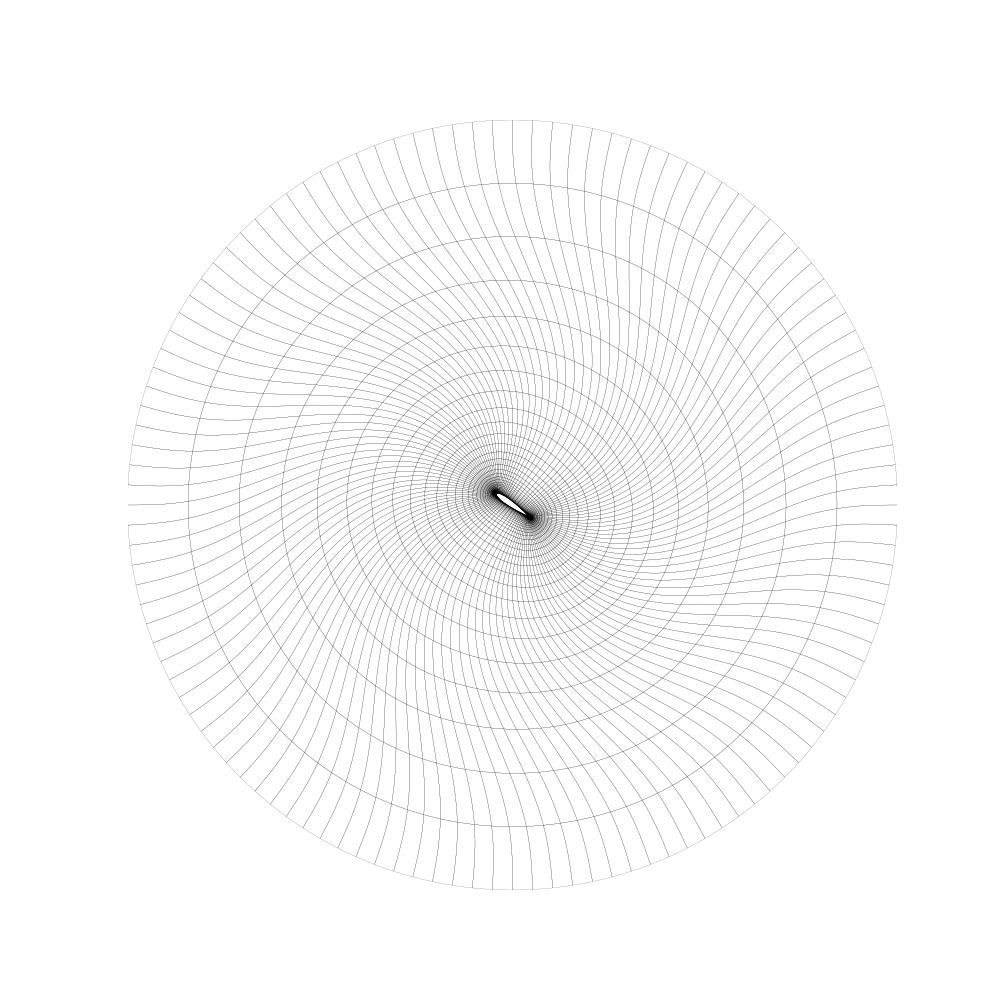
\includegraphics[width=0.85\textheight]{figs/domain}
  \end{center}
\end{frame}

\begin{frame}
  \frametitle{Parameter space}

  \begin{center}
    \begin{tikzpicture}[scale=6]
      \draw[very thick, ->] (0,0) -- (1,0);
      \draw[very thick, ->] (0,0) -- (0,1);
      \node[anchor=south west] at (0,0) {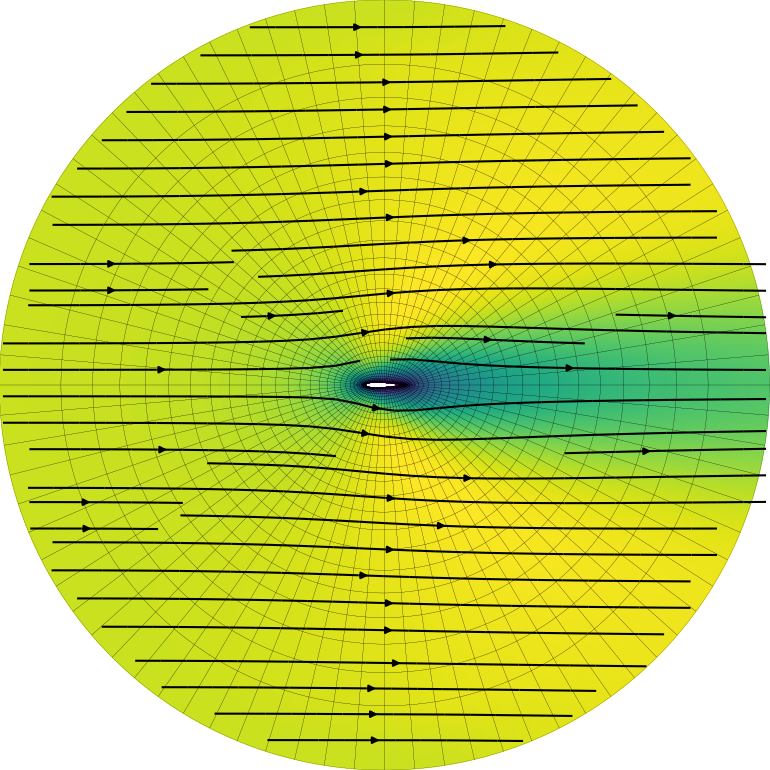
\includegraphics[width=28mm]{figs/full-lo-lo}};
      \node[anchor=south east] at (1,0) {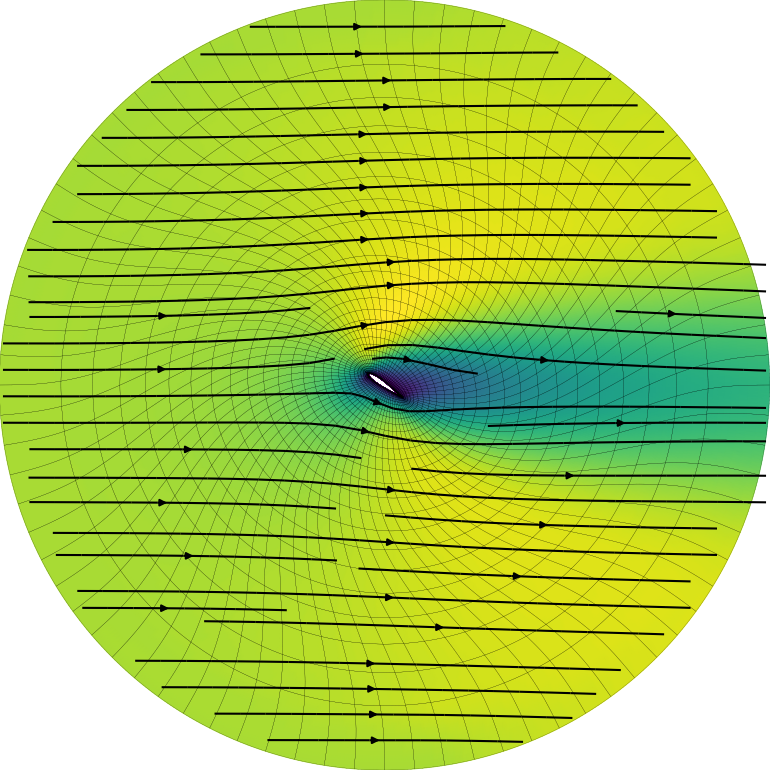
\includegraphics[width=28mm]{figs/full-hi-lo}};
      \node[anchor=north east] at (1,1) {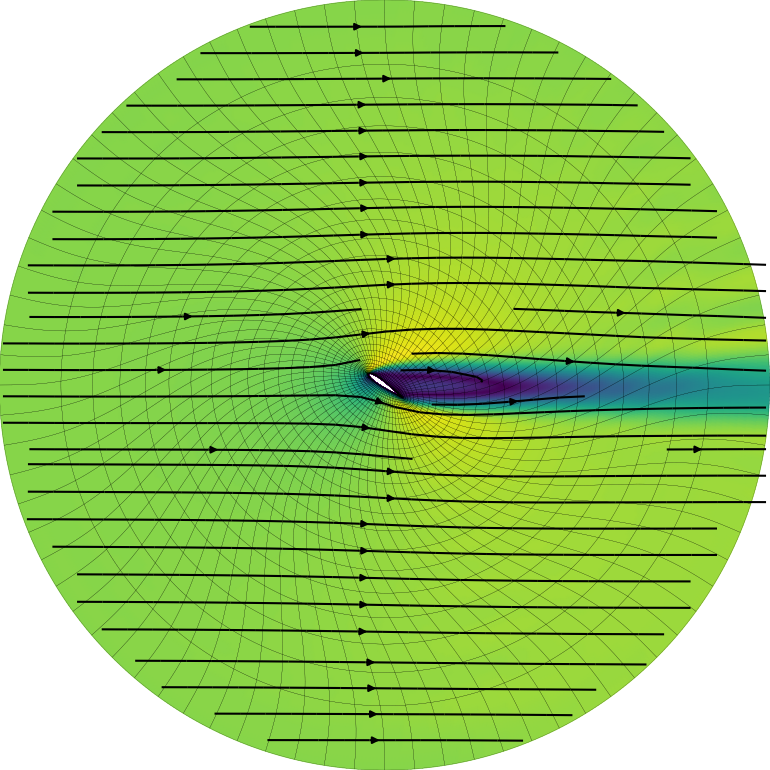
\includegraphics[width=28mm]{figs/full-hi-hi}};
      \node[anchor=north west] at (0,1) {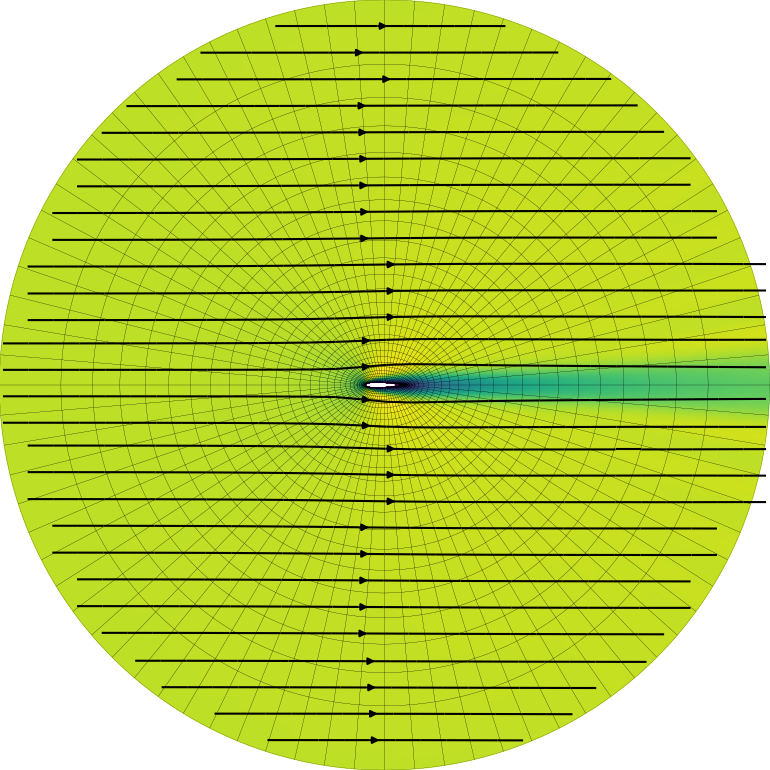
\includegraphics[width=28mm]{figs/full-lo-hi}};
      \node[anchor=north] at (0.5,0) {Angle of attack ($\varphi$)};
      \node[anchor=south, rotate=90] at (0,0.5) {Airspeed ($u_\infty$)};
    \end{tikzpicture}
  \end{center}
\end{frame}

\begin{frame}
  \frametitle{Affine representations}

  \begin{itemize}
  \item We will try two high-fidelity methods: a TH (1,2)-method and an IGA (1,2)
    divergence-conforming method.
  \item Not possible to express the Navier Stokes problem as finite sums
    \[
      \bm A_h(\bm \mu) = \textstyle \sum_i \xi_i(\bm \mu) \bm A_i, \qquad
      \bm f_h(\bm \mu) = \textstyle \sum_i \chi_i(\bm \mu) \bm f_i
    \]
  \item Instead, we use truncated series expansions.
  \item For a maximal angle of attack of $\SI{35}{\degree}$ we can expect about $10$ digits of
    accuracy with a reasonable number of terms \\ ($\sim 25$ for TH, $\sim 75$ for DC).
  \end{itemize}
\end{frame}

\begin{frame}
  \frametitle{Affine representations (TH)}

  \begin{align*}
    a(\hat{\bm u}, \hat{\bm w}; \varphi) &\approx \nu \int_{\hat{\Omega}}
      \nabla \hat{\bm u} : \left[ (1 + \varphi \bm D_1 - \varphi^2 \bm D_2) \nabla \right] \hat{\bm w} \\
    b(\hat{p}, \hat{\bm w}; \varphi) &\approx \sum_{i=0}^{2n} \varphi^i
    \int_{\hat{\Omega}} \hat{p} \bm B^{(-)}_i : \nabla \hat{\bm w} \\
  c(\hat{\bm u}, \hat{\bm v}, \hat{\bm w}; \varphi)
  &\approx \sum_{i=0}^{2n} \varphi^i \int_{\hat{\Omega}}
    (\hat{\bm u} \cdot \bm B^{(-)}_i \nabla) \hat{\bm v} \cdot \hat{\bm w}
  \end{align*}
\end{frame}

\begin{frame}
  \frametitle{Affine representations (TH)}

  \begin{align*}
    a(\hat{\bm u}, \hat{\bm w}; \varphi)
    &\approx \sum_{i,j=0}^{2n} \varphi^{i+j} \int_{\hat{\Omega}}
      \nabla (\bm B^{(+)}_i \hat{\bm u}) : \nabla (\bm B^{(+)}_j \hat{\bm w}) \\
    &+ \sum_{i,j=0}^{2n} \varphi^{i+j+1} \int_{\hat{\Omega}}
      \nabla (\bm B^{(+)}_i \hat{\bm u}) : (\bm D_1 \nabla) (\bm B^{(+)}_j \hat{\bm w}) \\
    &- \sum_{i,j=0}^{2n} \varphi^{i+j+2} \int_{\hat{\Omega}}
      \nabla (\bm B^{(+)}_i \hat{\bm u}) : (\bm D_2 \nabla) (\bm B^{(+)}_j \hat{\bm w}) \\
    b(\hat{p}, \hat{\bm w}; \varphi) &\approx \sum_{i,j=0}^{2n} \varphi^{i+j}
      \int_{\hat{\Omega}} \hat{p} \bm B^{(-)}_i :
      \nabla \left( \bm B^{(+)}_j \hat{\bm w} \right) \\
  c(\hat{\bm u}, \hat{\bm v}, \hat{\bm w}; \varphi)
  &\approx \sum_{i,j=0}^{2n} \varphi^{i+j}
    \int_{\hat{\Omega}} (\hat{\bm u} \cdot \nabla) \bm B^{(+)}_i \hat{\bm v} \cdot \bm B^{(+)}_j \hat{\bm w}
  \end{align*}
\end{frame}

\begin{frame}
  \begin{block}{\centering Our guiding principle}
    \begin{center}
      \vspace{5mm}
      All is fair in love, war and the offline stage. \\
      --- John Lyly (\emph{Euphues}; 1579)
      \vspace{5mm}
    \end{center}
  \end{block}
\end{frame}

\begin{frame}
  \frametitle{Ensembles}

  \begin{itemize}
  \item We calculated $15 \times 15$ solutions at the Gauss quadrature nodes.
  \item The parameter domain was chosen as
    \[
      \mathcal{P} = [-\SI{35}{\degree}, +\SI{35}{\degree}] \times
      [\SI{1}{\meter/\second}, \SI{20}{\meter/\second}].
    \]
  \item Only \emph{stationary} Navier-Stokes, with $\nu = \frac{1}{6}$.
  \end{itemize}
\end{frame}

\begin{frame}
  \frametitle{Spectrum}

  \begin{center}
    \begin{tikzpicture}
      \begin{axis}[
        xlabel={$k$},
        ylabel={$\lambda_k$},
        ymode=log,
        xmin=0, xmax=225,
        width=0.9\textwidth,
        height=0.6\textwidth,
        grid=both,
        axis lines=left,
        legend style={
          at={(1, 1)},
          anchor=north east,
          font=\small,
        },
        legend cell align=left,
        ]
        \addplot[red, thick]
        table[x index={0}, y index={1}]{data/airfoil-spectrum-no-piola.csv};
        \addplot[blue, thick]
        table[x index={0}, y index={2}]{data/airfoil-spectrum-no-piola.csv};
        \addplot[green, thick]
        table[x index={0}, y index={3}]{data/airfoil-spectrum-no-piola.csv};
        \addplot[red, thick, dashed]
        table[x index={0}, y index={1}]{data/airfoil-spectrum-piola.csv};
        \addplot[blue, thick, dashed]
        table[x index={0}, y index={2}]{data/airfoil-spectrum-piola.csv};
        \addplot[green, thick, dashed]
        table[x index={0}, y index={3}]{data/airfoil-spectrum-piola.csv};
        \legend{TH ($v$), TH ($p$), TH (sup), DC ($v$), DC ($p$), DC (sup)}
      \end{axis}
    \end{tikzpicture}
  \end{center}
\end{frame}

\begin{frame}
  \frametitle{Basis functions (v, TH, \only<1>{1}\only<2>{2}\only<3>{3}\only<4>{4})}

  \begin{center}
    \only<1>{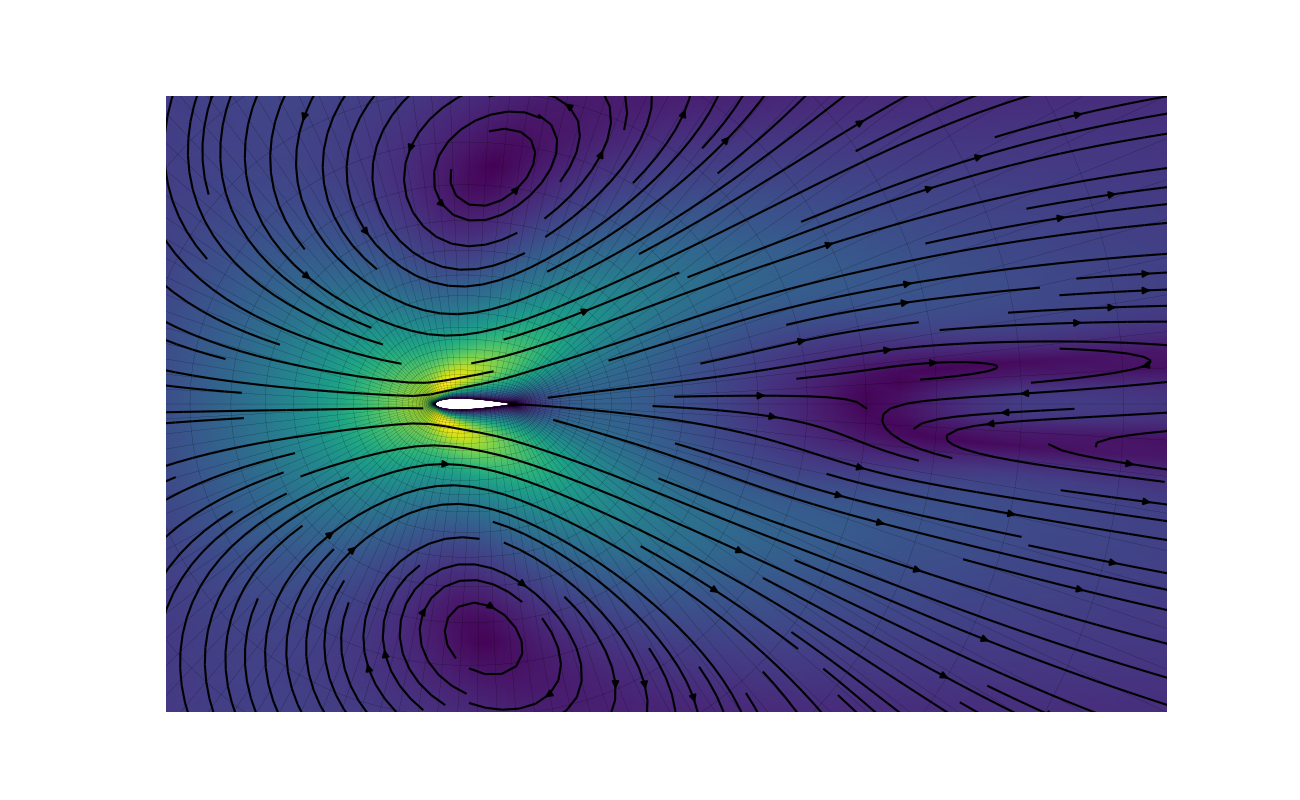
\includegraphics[width=0.8\textwidth]{figs/bfun-v-no-piola-v000}
    }\only<2>{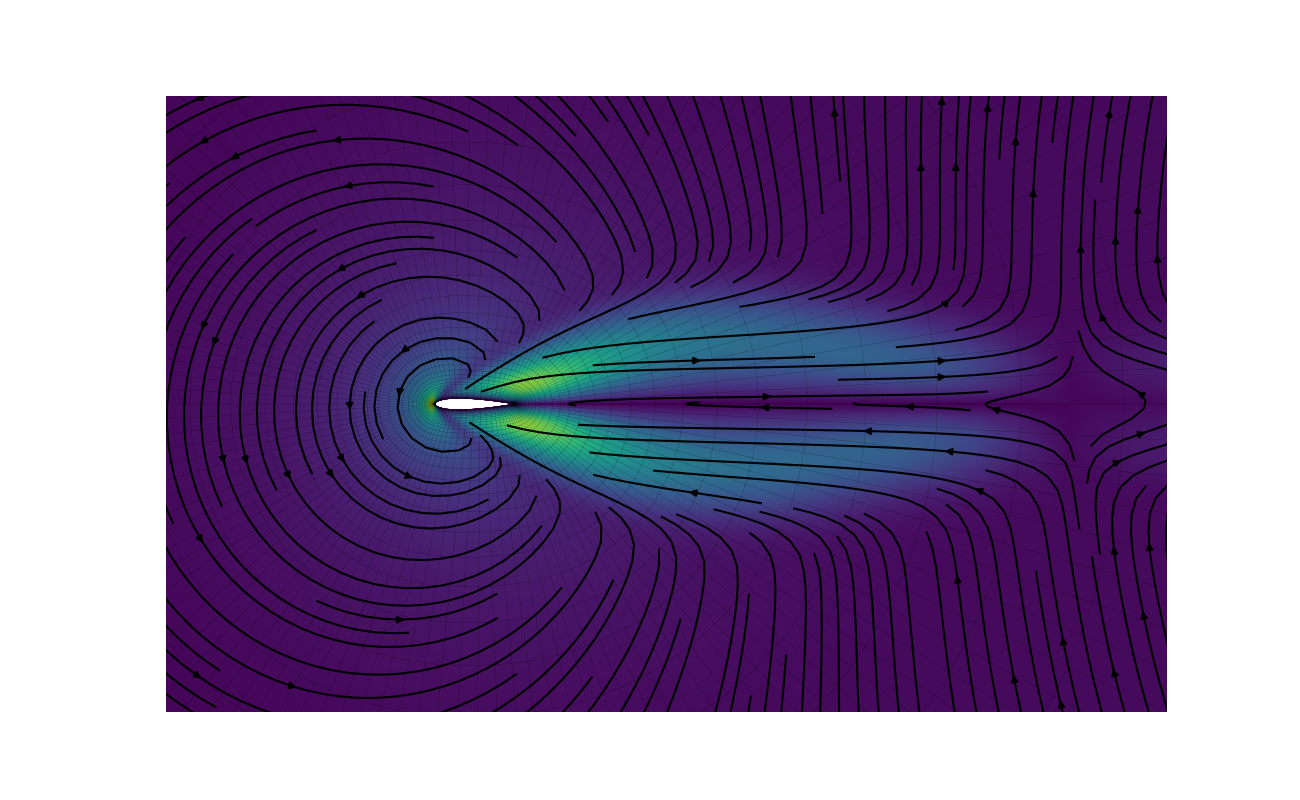
\includegraphics[width=0.8\textwidth]{figs/bfun-v-no-piola-v001}
    }\only<3>{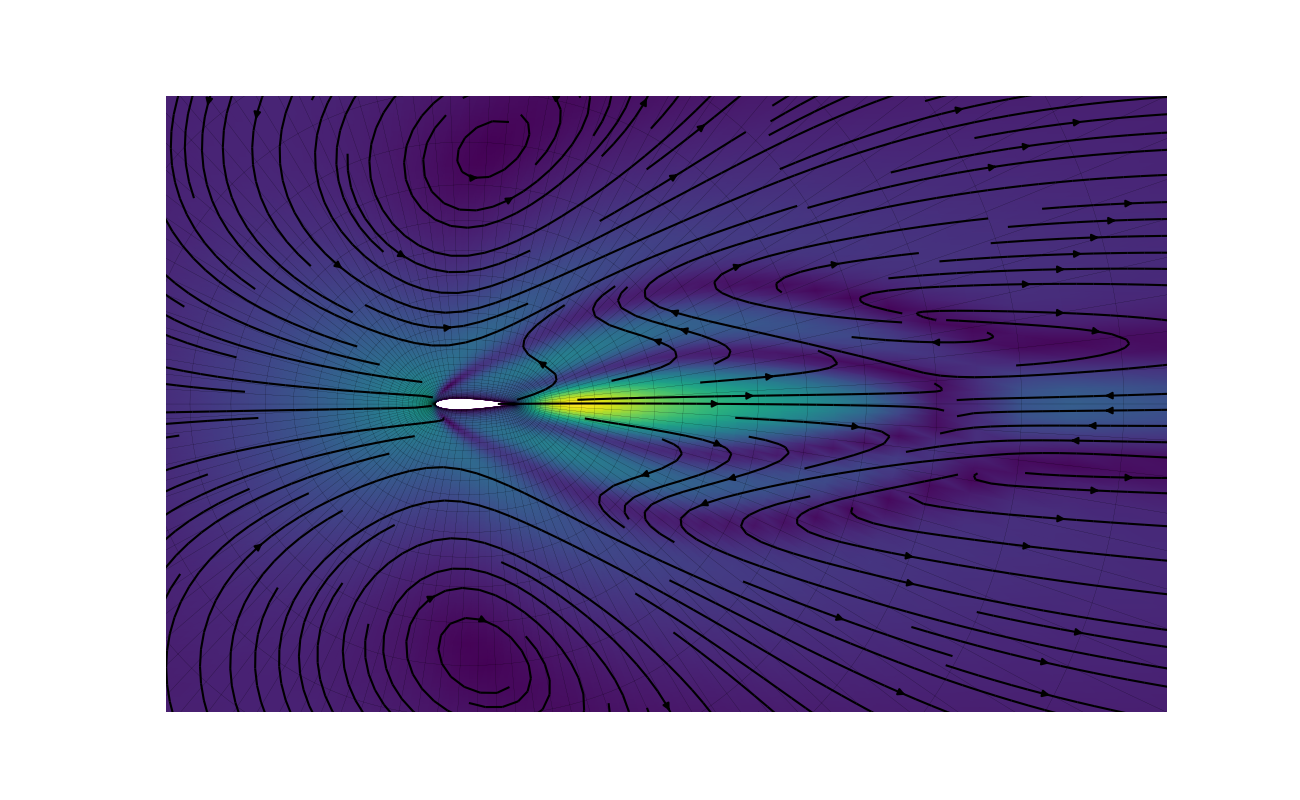
\includegraphics[width=0.8\textwidth]{figs/bfun-v-no-piola-v002}
    }\only<4>{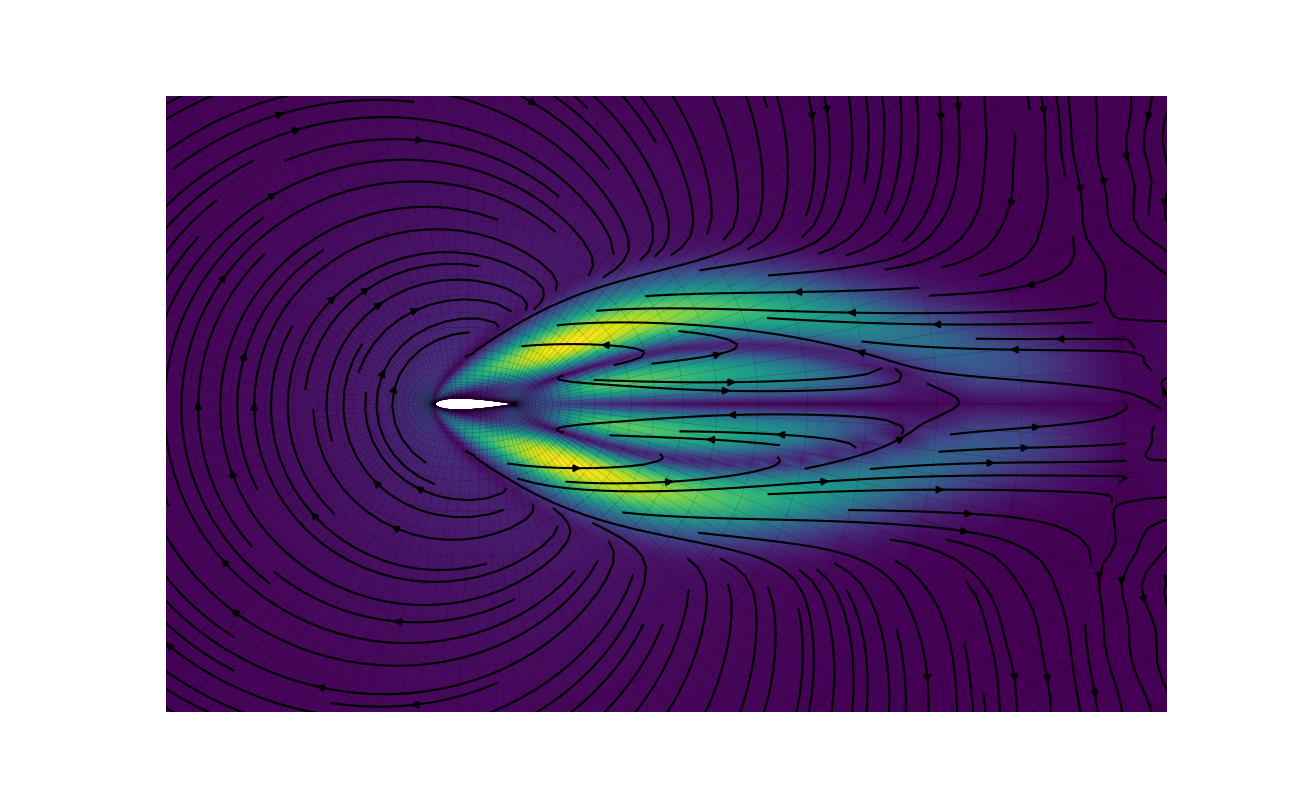
\includegraphics[width=0.8\textwidth]{figs/bfun-v-no-piola-v003}}
  \end{center}
\end{frame}

\begin{frame}
  \frametitle{Basis functions (v, DC, \only<1>{1}\only<2>{2}\only<3>{3}\only<4>{4})}

  \begin{center}
    \only<1>{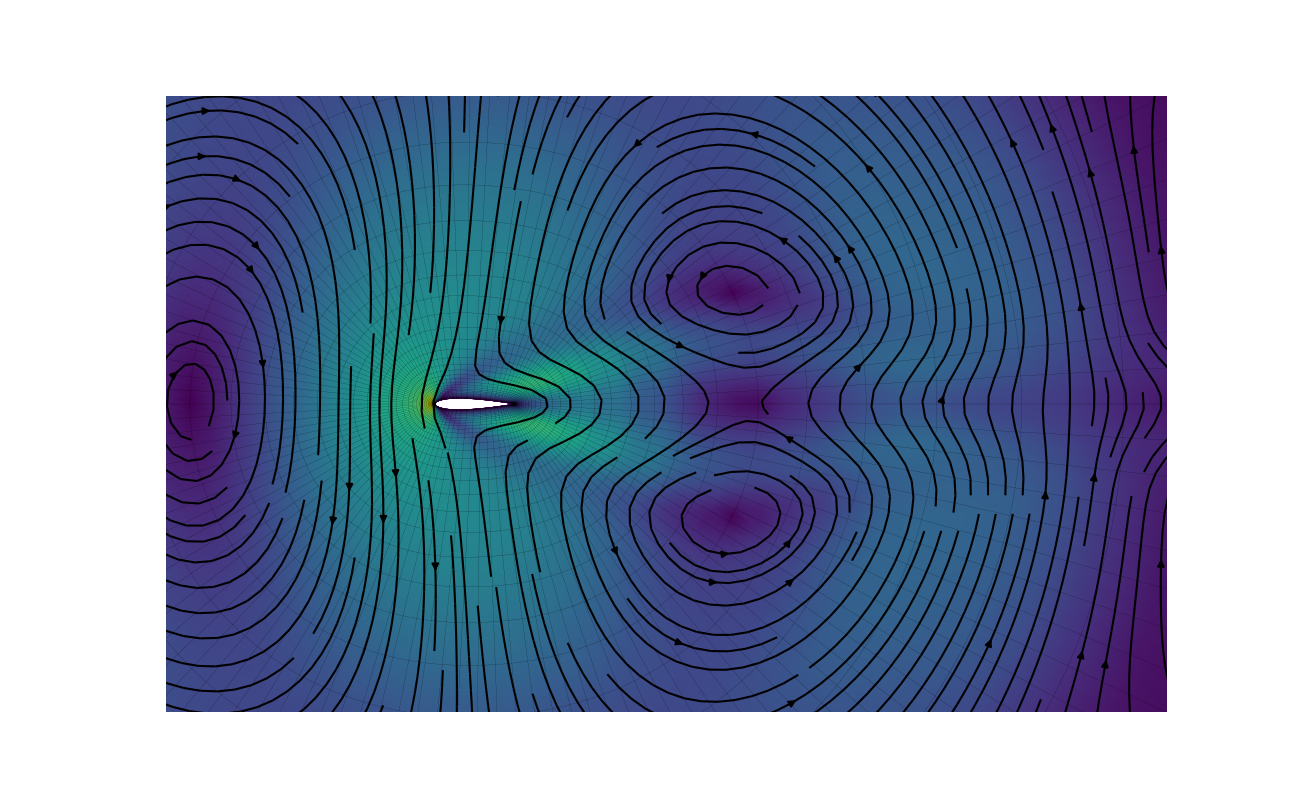
\includegraphics[width=0.8\textwidth]{figs/bfun-v-piola-v000}
    }\only<2>{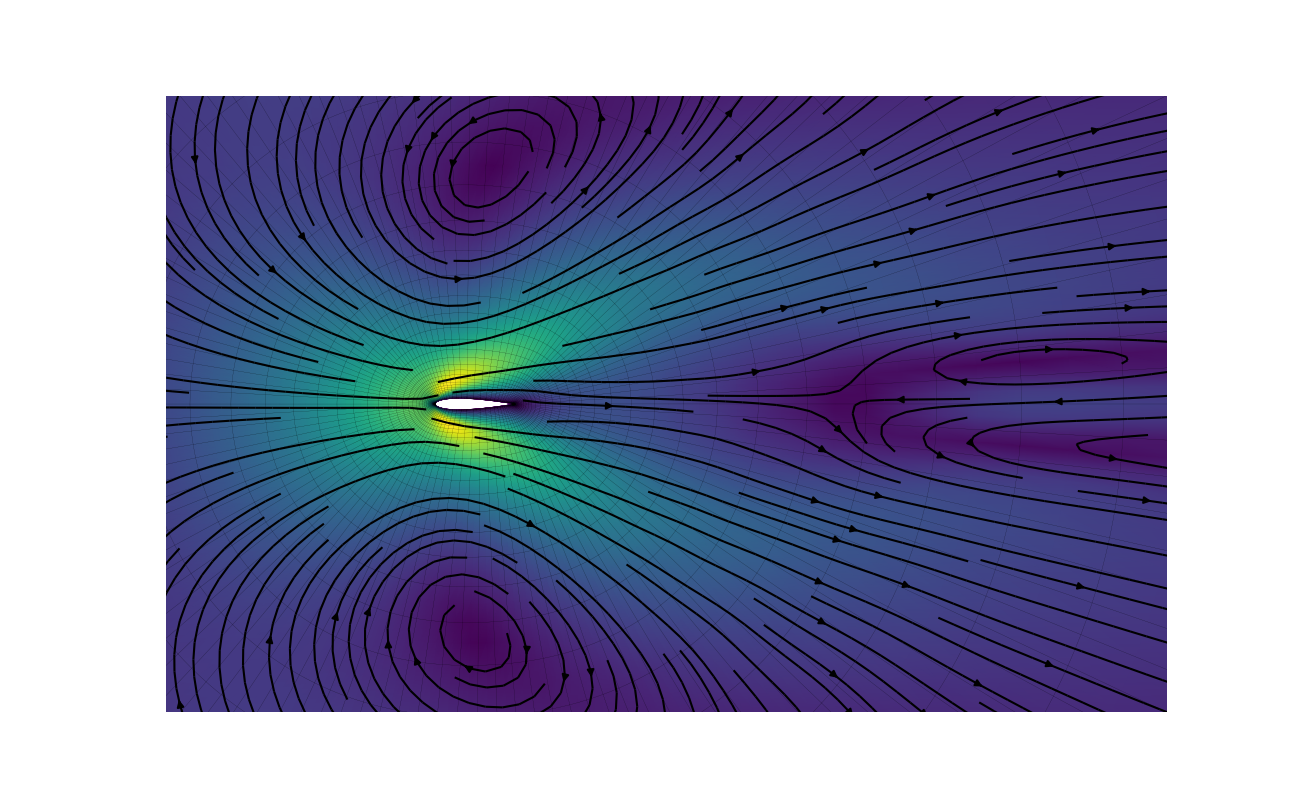
\includegraphics[width=0.8\textwidth]{figs/bfun-v-piola-v001}
    }\only<3>{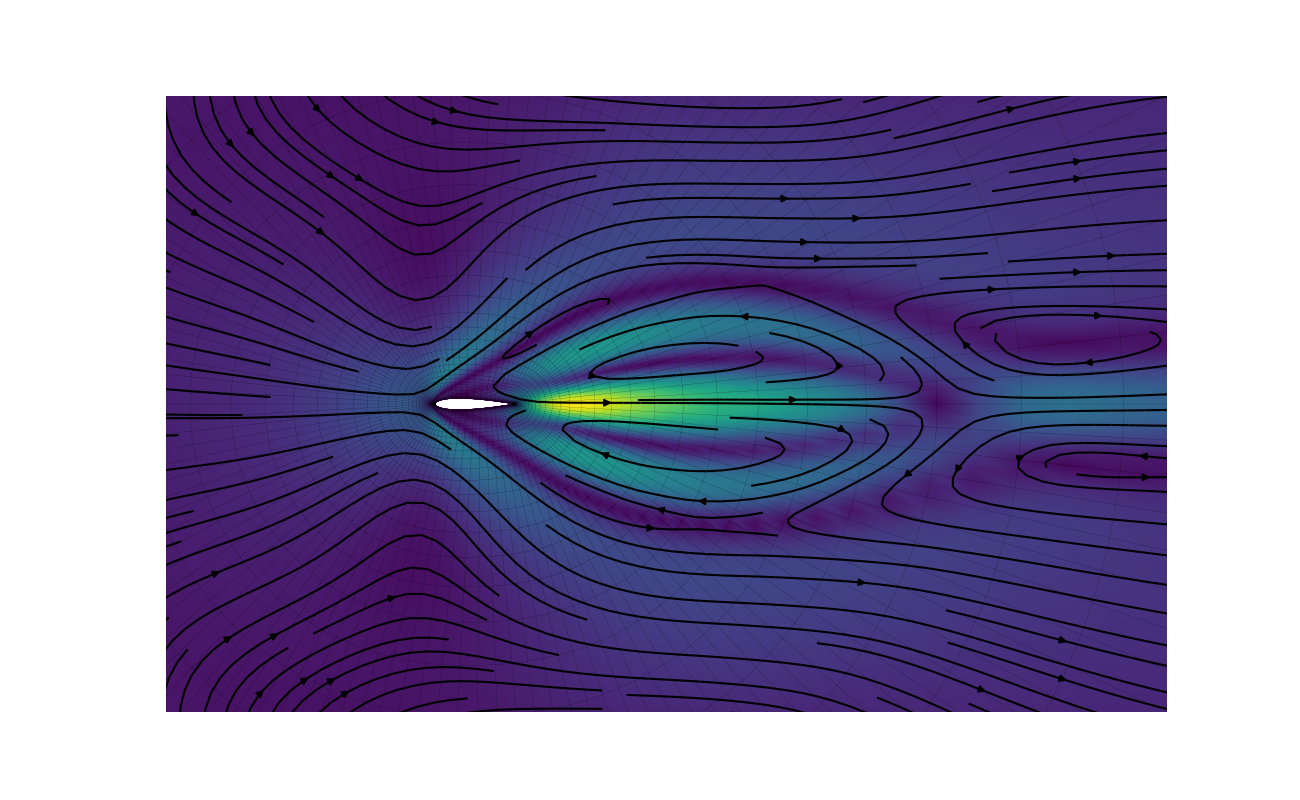
\includegraphics[width=0.8\textwidth]{figs/bfun-v-piola-v002}
    }\only<4>{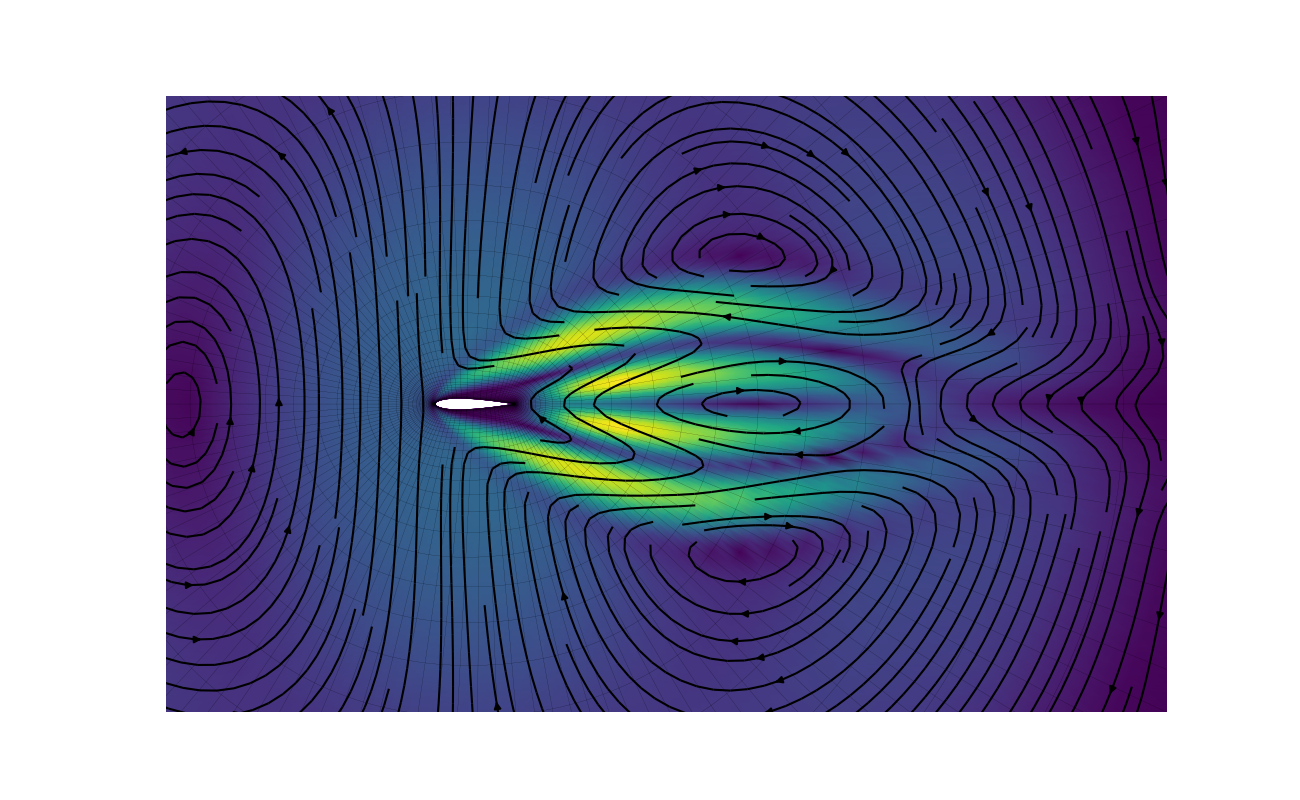
\includegraphics[width=0.8\textwidth]{figs/bfun-v-piola-v003}}
  \end{center}
\end{frame}

\begin{frame}
  \frametitle{Basis divergence}

  \begin{center}
    \begin{tikzpicture}
      \begin{axis}[
        xlabel={Angle of attack ($\varphi$, degrees)},
        ylabel={Divergence ($L^2$-norm)},
        ymode=log,
        width=0.9\textwidth,
        height=0.6\textheight,
        grid=both,
        axis lines=left,
        legend style={
          at={(0.5, -0.2)},
          anchor=north,
          draw=none,
        },
        legend cell align=left,
        legend columns=2,
        ]
        \addplot[blue, thick, mark=*, mark options={solid}]
        table[x index={0}, y index={2}]{data/airfoil-divs-no-piola.csv};
        \addplot[blue, thick, densely dashed, mark=o, mark options={solid}]
        table[x index={0}, y index={1}]{data/airfoil-divs-no-piola.csv};
        \addplot[red, thick, mark=*, mark options={solid}]
        table[x index={0}, y index={2}]{data/airfoil-divs-piola.csv};
        \addplot[red, thick, densely dashed, mark=o, mark options={solid}]
        table[x index={0}, y index={1}]{data/airfoil-divs-piola.csv};
        \legend{TH mean, TH max, DC mean, DC max}
      \end{axis}
    \end{tikzpicture}
  \end{center}
\end{frame}

\begin{frame}
  \frametitle{Convergence}

  \begin{center}
    \begin{tikzpicture}
      \begin{axis}[
        xlabel={Expected mean relative error},
        ylabel={Mean relative error},
        ymode=log,
        xmode=log,
        width=0.9\textwidth,
        height=0.5\textwidth,
        grid=both,
        axis lines=left,
        legend style={
          at={(0.5, -0.3)},
          anchor=north,
          draw=none,
        },
        legend cell align=left,
        legend columns=4,
        ]
        \addplot[blue, thick, mark=*, mark options={solid}]
        table[x index={1}, y index={4}]{data/airfoil-results-no-piola-sups-no-block.csv};
        \addplot[blue, thick, densely dashed, mark=o, mark options={solid}]
        table[x index={2}, y index={8}]{data/airfoil-results-no-piola-sups-no-block.csv};
        \addplot[red, thick, mark=*, mark options={solid}]
        table[x index={1}, y index={4}]{data/airfoil-results-piola-sups-no-block.csv};
        \addplot[red, thick, densely dashed, mark=o, mark options={solid}]
        table[x index={2}, y index={8}]{data/airfoil-results-piola-sups-no-block.csv};
        \legend{TH ($v$), TH ($p$), DC ($v$), DC ($p$)}
      \end{axis}
    \end{tikzpicture}
  \end{center}
\end{frame}

\begin{frame}
  \frametitle{Convergence}

  \begin{center}
    \begin{tikzpicture}
      \begin{axis}[
        xlabel={Degrees of freedom ($M$)},
        ylabel={Mean relative error},
        ymode=log,
        width=0.9\textwidth,
        height=0.5\textwidth,
        grid=both,
        axis lines=left,
        legend style={
          at={(0.5, -0.3)},
          anchor=north,
          draw=none,
        },
        legend cell align=left,
        legend columns=4,
        ]
        \addplot[blue, thick, mark=*, mark options={solid}]
        table[x index={0}, y index={4}]{data/airfoil-results-no-piola-sups-no-block.csv};
        \addplot[blue, thick, densely dashed, mark=o, mark options={solid}]
        table[x index={0}, y index={8}]{data/airfoil-results-no-piola-sups-no-block.csv};
        \addplot[red, thick, mark=*, mark options={solid}]
        table[x index={0}, y index={4}]{data/airfoil-results-piola-sups-no-block.csv};
        \addplot[red, thick, densely dashed, mark=o, mark options={solid}]
        table[x index={0}, y index={8}]{data/airfoil-results-piola-sups-no-block.csv};
        \legend{TH ($v$), TH ($p$), DC ($v$), DC ($p$)}
      \end{axis}
    \end{tikzpicture}
  \end{center}
\end{frame}

\begin{frame}
  \frametitle{Convergence}

  \begin{center}
    \begin{tikzpicture}
      \begin{axis}[
        xlabel={Time (seconds)},
        ylabel={Mean relative error},
        ymode=log,
        xmode=log,
        width=0.9\textwidth,
        height=0.5\textwidth,
        grid=both,
        axis lines=left,
        legend style={
          at={(0.5, -0.3)},
          anchor=north,
          draw=none,
        },
        legend cell align=left,
        legend columns=4,
        ]
        \addplot[blue, thick, mark=*, mark options={solid}]
        table[x index={15}, y index={4}]{data/airfoil-results-no-piola-sups-no-block.csv};
        \addplot[blue, thick, densely dashed, mark=o, mark options={solid}]
        table[x index={15}, y index={8}]{data/airfoil-results-no-piola-sups-no-block.csv};
        \addplot[red, thick, mark=*, mark options={solid}]
        table[x index={15}, y index={4}]{data/airfoil-results-piola-sups-block.csv};
        \addplot[red, thick, densely dashed, mark=o, mark options={solid}]
        table[x index={15}, y index={8}]{data/airfoil-results-piola-sups-block.csv};
        \legend{TH ($v$), TH ($p$), DC ($v$), DC ($p$)}
      \end{axis}
    \end{tikzpicture}
  \end{center}
\end{frame}

\begin{frame}
  \frametitle{Summary}
  \begin{itemize}
  \item Reduced order models can offer dramatic speed-ups for certain applications.
  \item They combine nicely with IGA and div-compatible spaces to form fully
    divergence-free function spaces without need for pressure fields.
  \item Divergence-free RBMs can be much faster than other RBMs, in spite of additional complexity
    in the offline stage (remember, all is fair there.)
  \end{itemize}
  ~\\ \begin{center} Thanks! \end{center}
\end{frame}

\end{document}
